\documentclass[a4paper, 12pt]{article}
\usepackage{graphicx}
\PassOptionsToPackage{hyphens}{url}\usepackage[hidelinks]{hyperref}
\usepackage{amsmath, amssymb}
\usepackage{geometry}
\usepackage{booktabs}
\usepackage{overpic}
\usepackage{pdfcomment} 
\usepackage{subcaption}

% Set the page geometry
\geometry{a4paper, margin=1in}

% Title and author information
\title{Computational Model Evaluation for Urban Microclimate Simulations}
\author{SMARTLab}
\date{\today}

% Bibliography management
\usepackage[style=mla-new,eprint=true,backend=bibtex,citestyle=authoryear]{biblatex}
\addbibresource{bibliography.bib}
\setlength\bibitemsep{1.5\baselineskip}


\begin{document}

%-------------------- Title -------------------------------------------------------------

\maketitle

%-------------------- Abstract ----------------------------------------------------------
\begin{abstract}
\noindent
This document presents a structured approach for the evaluation of computational models used in urban microclimate simulations. It serves two main purposes:
\begin{itemize}
    \item To outline a hierarchical validation strategy that decomposes the problem into subproblems, benchmarks, and test cases, using both controlled experimental and real-world datasets to ensure accuracy and reliability;
    \item To provide an up-to-date inventory of publicly available test cases relevant to computational model evaluation in the urban microclimate domain.
\end{itemize}
\end{abstract}

%------------------- Table of Contents --------------------------------------------------

\tableofcontents

%------------------- Sections -----------------------------------------------------------

\section{Introduction}
Urban microclimate simulations play a pivotal role in assessing environmental conditions such as pollutant dispersion and thermal behavior within urban areas. These simulations are essential for urban planning, public health, and sustainability efforts.

This document introduces a systematic evaluation methodology aimed at ensuring that computational models can reliably and accurately replicate the physical phenomena relevant to urban environments.

Model evaluation refers to the comprehensive process of determining how well a simulation model represents real-world processes. It encompasses both qualitative and quantitative comparisons between model predictions and empirical observations, and includes aspects such as model validation, performance assessment, and uncertainty quantification.

The validation strategy adopted here employs a hierarchical structure, specifically designed for the Atmospheric Boundary Layer (ABL) with urban micro-scale dynamics. This strategy includes:

\begin{itemize}
    \item Comparisons between simulation outputs and results with relevant observations from wind tunnel and field experiments;
    \item Statistical evaluations of model accuracy;
    \item Sensitivity analyses to assess robustness across model configurations and environmental scenarios.
\end{itemize}

\subsection{Atmospheric Boundary Layer}
ABL is classified into three idealized regimes: Neutrally Stratified Boundary Layer (NSBL), Stable Boundary Layer (SBL), and Convective Boundary Layer (CBL). Each of these regimes is characterized by different stability conditions that significantly influence urban microclimate behavior.

NSBL conditions are most compatible with available wind tunnel datasets but rarely occur in natural settings. SBL and CBL regimes, on the other hand, dominate the diurnal cycle of the urban boundary layer and are better captured in field measurements (and also in some specifically designed wind tunnels).

\begin{figure}[h!]
    \centering
    \begin{minipage}{0.47\textwidth}
        \centering
        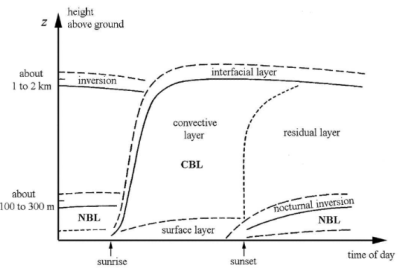
\includegraphics[width=\textwidth]{imgs/abl_cycle.png}
    \end{minipage}
    \hfill
    \begin{minipage}{0.47\textwidth}
        \centering
        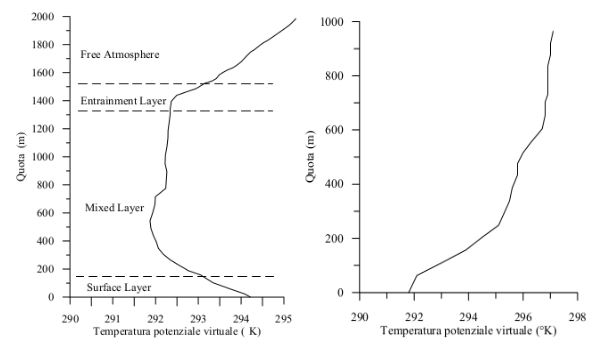
\includegraphics[width=\textwidth]{imgs/wind_speed_cycle.png}
    \end{minipage}
    \caption{Temporal evolution of the ABL and representative wind speed profile across a diurnal cycle.}
\end{figure}

\subsection{CFD Evaluation for Urban Microclimate Simulations}
Computational Fluid Dynamics (CFD) is a key tool for simulating airflow and pollutant dispersion in urban settings. These simulations provide detailed insight into microscale atmospheric behavior, but the reliability of CFD predictions strongly depends on rigorous model validation.

To ensure robustness and credibility, CFD models must be evaluated through a structured process that considers accuracy, computational efficiency, and physical fidelity. The hierarchical validation strategy introduced here supports these objectives by organizing test cases according to geometric complexity and atmospheric conditions.

The methodology leverages test cases derived from well-documented datasets, enabling focused evaluation of specific flow features and physical processes. Key goals of this strategy include:

\begin{itemize}
    \item Establishing a balance between computational cost and predictive accuracy;
    \item Validating models under different configurations of the ABL;
    \item Testing performance on canonical unit problems, such as flow over isolated buildings, through street canyons, and within complex topographies.
    \item Testing performance on real-world scenarios, such as urban areas with complex geometries and varying atmospheric conditions.
\end{itemize}

\noindent
Above-mentioned unit problems are designed to represent simplified, yet physically meaningful, urban scenarios in which buildings and other geometrical features are fully immersed in a turbulent boundary layer with dispersion of gaseous substances. The following categories are used:

\begin{itemize}
    \item Flow field around a \textbf{single building};
    \item Flow field within a \textbf{street canyon};
    \item \textbf{Dispersion} of neutrally and non-neutrally buoyant substances;
    \item Flow around \textbf{complex urban topographies}.
\end{itemize}

\begin{figure}[h!]
    \centering
    \begin{minipage}{0.44\textwidth}
        \centering
        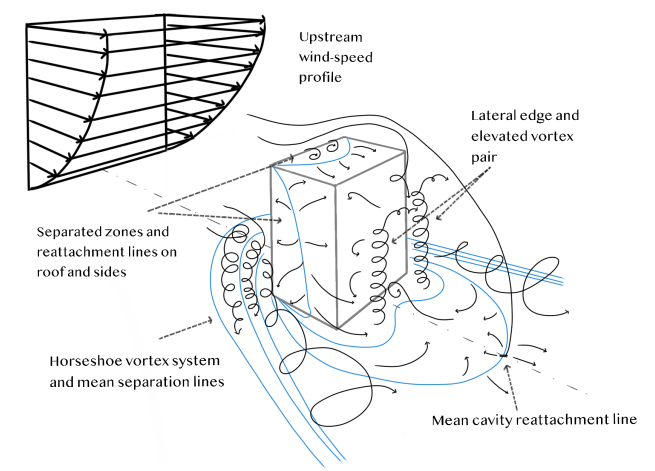
\includegraphics[width=\textwidth]{imgs/unit_problem_2.png}
    \end{minipage}
    \hfill
    \begin{minipage}{0.44\textwidth}
        \centering
        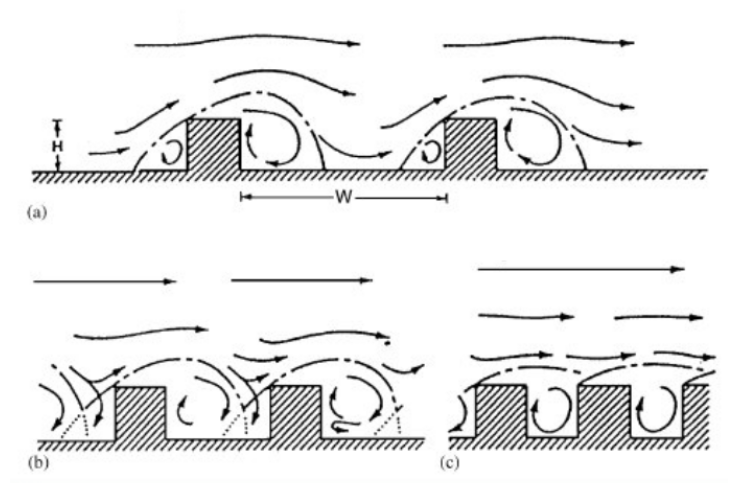
\includegraphics[width=\textwidth]{imgs/unit_problem_1.png}
    \end{minipage}
    \caption{Illustration of unit problems representing key physical phenomena in urban microclimates.}
\end{figure}


\section{Validation Strategy}

\subsection{Definition}
Regarding validation processes related to complex systems, \textcite{Oberkampf2010} suggested using a building block or system complexity hierarchy approach due to the infeasibility of true validation on most complex systems. 

This document adopts that hierarchical strategy, organizing model evaluation across progressively challenging scenarios, ranging from simplified geometries in controlled and simplified conditions to real-world urban environments. This allows to assess the accuracy of the computational results compared with the experimental data at multiple degrees of physics coupling and geometric complexity.\newline

Validation strategy decomposes the problem into subproblems of increasing complexity, exploiting the possible configurations of the ABL and the unitary problems concerning urban dispersion phenomena.\newline

Validation procedure takes into account available datasets related to atmospheric dispersion modelling in micro-scale environments. These validation data for numerical models must fulfil specific requirements with respect to completeness, spatial and temporal resolution, accuracy, representativeness, and the documentation of the measured results must be available \parencite{Chang2003}.

\subsection{Comparative analyses}

For each dataset, an OpenFOAM test case is developed to enable a consistent suite of comparative analyses. These analyses serve both general and case-specific purposes.\newline

\noindent
General objectives for all test cases include:
\begin{itemize}
    \item Performing grid sensitivity studies to assess numerical resolution dependence;
    \item Conducting sensitivity analyses on turbulence models and numerical schemes;
    \item Exploring transitions from full-order to reduced-order modeling approaches;
    \item Replacing experimental boundary conditions with reconstructed inflow profiles
\end{itemize}


\subsection{Assessment of the results}
Model performance is assessed by comparing simulation results to experimental datasets. The validation process focuses on:
\begin{itemize}
    \item Quantitative metrics comparing point-wise scalar values (e.g., velocity magnitude, temperature, pollutant concentration);
    \item Qualitative representation of results with 2D and 3D plots to aid interpretation and model comparison.
\end{itemize}

\noindent
Each test case includes the computation of statistical metrics, detailed in \ref{sec:statistical_metrics}. An example of the post-processing procedure is provided to illustrate the analysis of simulation results (see Section \ref{sec:post_processing}).

\subsubsection{Statistical metrics \label{sec:statistical_metrics}}
Quantitative comparison of experimental and model results is performed using the following statistical performance measures (where $P_i$ is the model prediction, $O_i$ is the observed value):
\begin{description}

    \item[Geometric mean bias $\;\left( MG \right)$ :] is the logarithmic measure of the mean relative bias thus is strongly influenced by extremely low observations and predictions for the concentrations.It is not so strongly influenced by infrequently occurring high observations and pre dictions for the concentrations as the fractional bias.It indicates only systematic errors. For an ideal model MG=1. 

    \begin{equation*}
        MG = \mbox{exp}\;(\,\frac{1}{n}\;\sum_{i=1}^n\mbox{ln} O_i - \frac{1}{n}\;\sum_{i=1}^n\mbox{ln} P_i\,)
    \end{equation*}

    \item[Geometric variance $\;\left( VG \right)$ :] is a metric like the NMSE, it shows the scatter in the data and therefore contains both, systematic and random errors. For an ideal model prediction one would have VG=1.

    \begin{equation*}
        VG\;=\;\mbox{exp}\,\left[\,\frac{1}{n}\;\sum_{i=1}^n(\mbox{ln}\,O_i - \mbox{ln}\,P_i)^2\,\right]
    \end{equation*}

    \item[Normalised mean square error $\;\left( NMSE \right)$ :] is a measure of the scatter of the data and therefore indicates both, systematic and random errors. For an ideal model prediction one would have NMSE=0. NMSE makes no sense for parameters that can take both positive and negative values, such as velocity components.

    \begin{equation*}
        NMSE\;=\;\frac{1}{n}\;\sum_{i=1}^n\;\frac{(\;O_i - P_i\;)^2}{\overline{O}\;\overline{P}}
    \end{equation*}

    \item[Normalised relative error $\;\left( NRE_i \right)$ :] is a local measure of the relative difference between predicted and observed values, computed at each spatial point $i$. It is typically used to generate visualisations, such as 3D error plots.

\begin{equation*}
    NRE_i = \left| \frac{P_i - O_i}{O_i} \right| \times 100
\end{equation*}

\end{description}

\clearpage

\subsubsection{Post-processing example \label{sec:post_processing}}

Here we provide an example of the basic post-processing available for each test case that belongs to the validation procedure.

\begin{table}[ht]
    \centering
    \begin{tabular}{r|cc|cc|cc}  
        \toprule
        \textbf{Case} & \multicolumn{2}{c|}{\textbf{NMSE}} & \multicolumn{2}{c|}{\textbf{MG}} & \multicolumn{2}{c}{\textbf{GV}} \\
                     & UMag & k                           & UMag & k                         & UMag & k \\
        \midrule
        Case-A & 0.030 & 1.342 & 1.013 & 2.067 & 1.262 & 2.761 \\
        Case-B & 0.030 & 1.341 & 1.011 & 2.067 & 1.264 & 2.763 \\
        Case-C & 0.023 & 1.603 & 0.991 & 2.266 & 1.251 & 3.462 \\
        Case-D & 0.027 & 1.345 & 1.012 & 2.087 & 1.252 & 2.845 \\
        Case-E & 0.034 & 1.297 & 0.964 & 2.035 & 1.227 & 2.907 \\
        \bottomrule
    \end{tabular}
    \caption{Tabular data of statistical metrics - Comparison of multiple
        simulations data at the end}
    \label{tab:statistics}
\end{table}

\begin{figure}[h!]
    \centering
    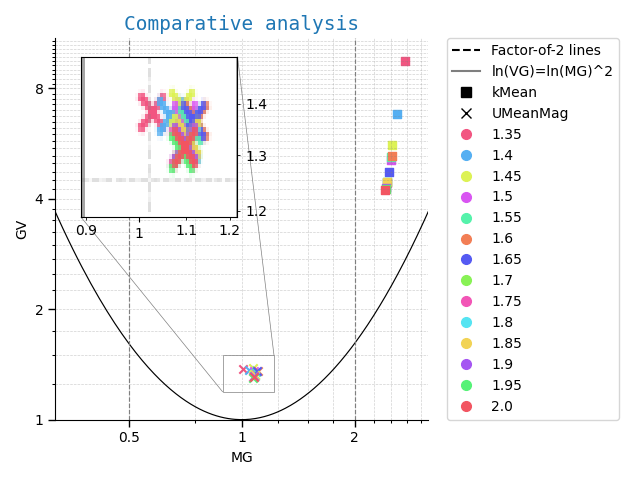
\includegraphics[width=0.9\textwidth]{imgs/quantitative_package_single.png}
    \caption{Graphical representation of statistical metrics - comparison of single 
        simulation data over time}
    \vspace*{-0.5cm}
    \label{example_quantitative} 
\end{figure}

\begin{figure}[h!]
    \centering
    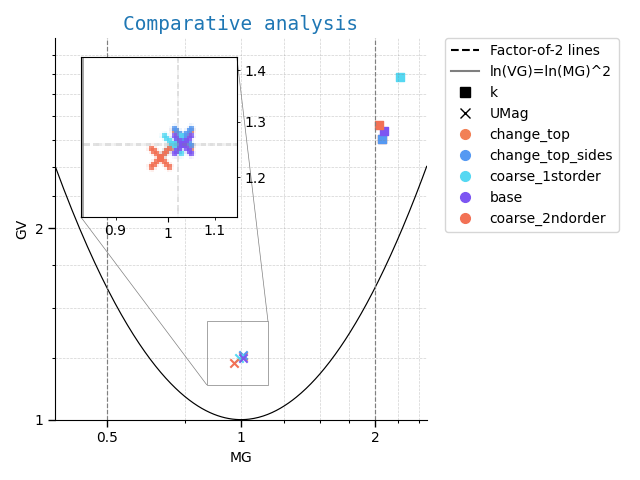
\includegraphics[width=0.9\textwidth]{imgs/quantitative_package_multi.png}
    \caption{Graphical representation of statistical metrics - Comparison of multiple
        simulations data at the end}
    \vspace*{-0.5cm}
    \label{example_quantitative} 
\end{figure}

\newpage

\begin{figure}[h!]
    \centering
    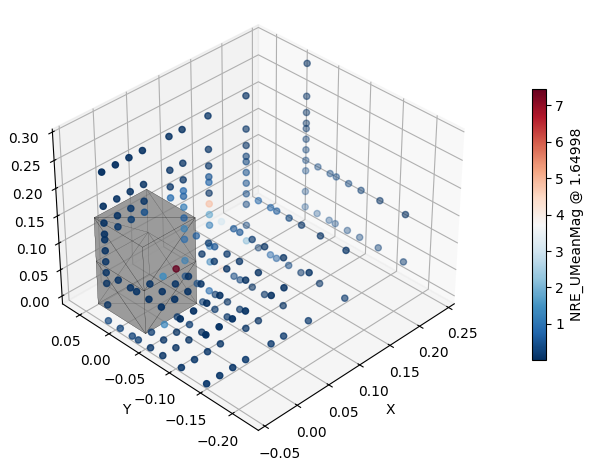
\includegraphics[width=0.8\textwidth]{imgs/3dplot_nre_example.png}
    \caption{3D plot of Normalised Relative Error (NRE)}
    \vspace*{-0.5cm}
    \label{example_3dplot}
\end{figure}

\begin{figure}[h!]
    \centering
    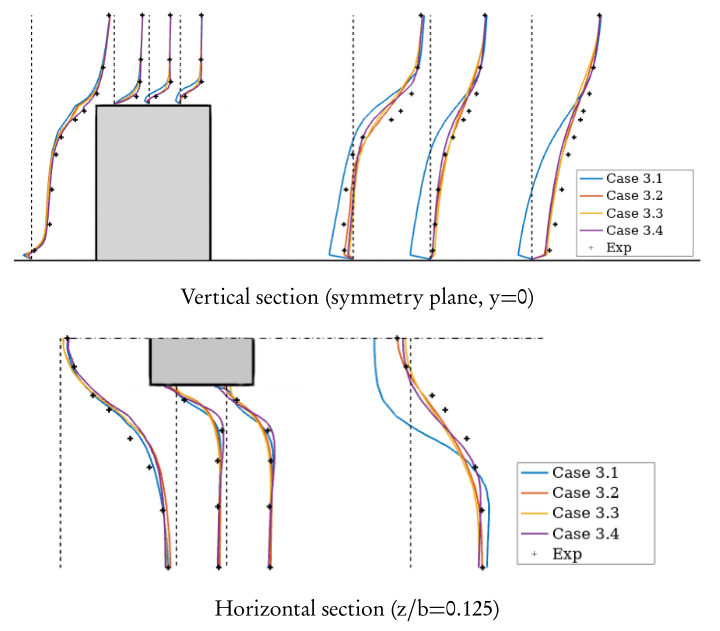
\includegraphics[width=1.0\linewidth]{imgs/qualitative_package.png}
    \caption{Comparison of multiple simulations results line data}
    \label{Line data visualization along with experiment point data}
\end{figure}


\clearpage

\subsection{Validation Strategy Diagram}
Here follow the proposed validation hierarchy with the up-to-date selected test cases to be simulated.
\vspace*{-1cm}
\begin{figure}[h!]
    \centering
    \begin{overpic}[width=\textwidth]{imgs/block_diagram.pdf}
        \put(7.8,30){\hyperlink{link:aij_A}{\makebox[3cm][l]{\rule{0pt}{0.5cm}}}}
        \put(7.8,26.3){\hyperlink{link:sef_A}{\makebox[3cm][l]{\rule{0pt}{0.5cm}}}}
        \put(7.8,22.5){\hyperlink{link:aij_C}{\makebox[3cm][l]{\rule{0pt}{0.5cm}}}}
        \put(7.8,19){\hyperlink{link:cost_c_wt}{\makebox[3cm][l]{\rule{0pt}{0.5cm}}}}
        \put(17.8,30){\hyperlink{link:tpu_A}{\makebox[3cm][l]{\rule{0pt}{0.5cm}}}}
        \put(17.8,26.3){\hyperlink{link:sef_A}{\makebox[3cm][l]{\rule{0pt}{0.5cm}}}}
        \put(17.8,22.5){\hyperlink{link:cost_m}{\makebox[3cm][l]{\rule{0pt}{0.5cm}}}}
        \put(31.8,30){\hyperlink{link:sef_A}{\makebox[3cm][l]{\rule{0pt}{0.5cm}}}}
        \put(31.8,26.3){\hyperlink{link:sef_A}{\makebox[3cm][l]{\rule{0pt}{0.5cm}}}}
        \put(50.8,30){\hyperlink{link:tpu_C}{\makebox[3cm][l]{\rule{0pt}{0.5cm}}}}
        \put(50.8,26.3){\hyperlink{link:sef_A}{\makebox[3cm][l]{\rule{0pt}{0.5cm}}}}
        \put(50.8,22.5){\hyperlink{link:sef_A}{\makebox[3cm][l]{\rule{0pt}{0.5cm}}}}
        \put(26,8){\hyperlink{link:cost_c_f}{\makebox[3cm][l]{\rule{0pt}{0.5cm}}}}
        \put(36,8){\hyperlink{link:turb_p}{\makebox[3cm][l]{\rule{0pt}{0.5cm}}}}
    \end{overpic}
    \vspace*{-1cm}
    \caption{Tiers representation of the validation strategy (All test cases refer to datasets described in the following sections, i.e. AIJ, TPU, SEF, COST, and TURB). }
    \label{validation_strategy} 
\end{figure}



\section{Datasets Overview}
Datasets considered by the validation procedure, already mentioned in the validation block diagram (Figure \ref{validation_strategy}).

\subsection{AIJ Dataset}
\url{https://www.aij.or.jp/jpn/publish/cfdguide/index_e.htm}\newline
% \begin{figure}[h!]
%     \centering
%     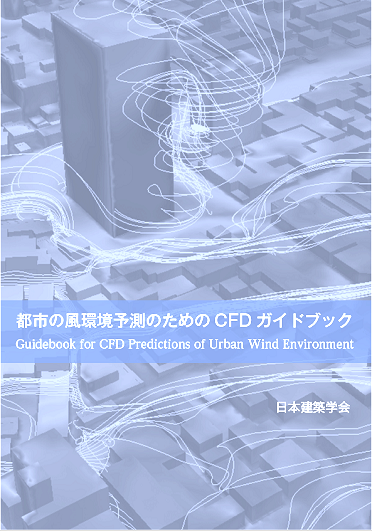
\includegraphics[scale=0.5]{imgs/aij_dataset_image.png}
%     \caption{For comparative analysis with respect to AIJ-A and AIJ-C}
% \end{figure}

\subsection{TPU Dataset}
\url{https://www.wind.arch.t-kougei.ac.jp/info_center/pollution/pollution.html}\newline
% \begin{figure}[h!]
%     \centering
%     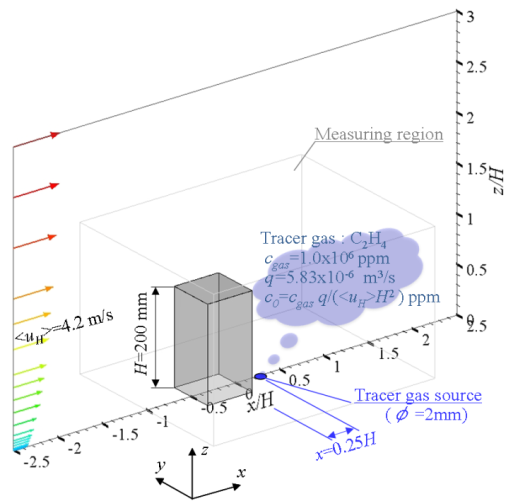
\includegraphics[scale=0.35]{imgs/tpu_dataset_image.png}
%     \caption{For comparative analysis TPU-A and TPU-B.} 
% \end{figure}

\subsection{StratEnFlo Dataset}
\url{https://figshare.com/articles/dataset/Array_of_buildings_with_incoming_stra-tification/8320007}\newline
% \vspace*{-0.2cm}\begin{figure}[h!]
%     \centering
%     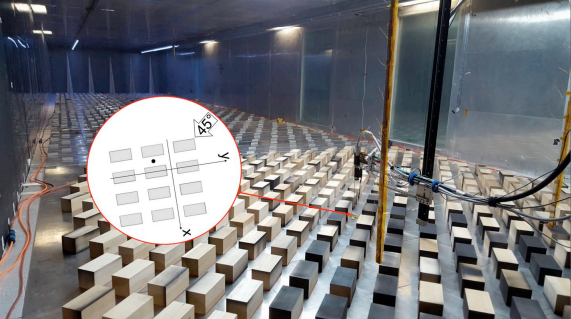
\includegraphics[scale=0.4]{imgs/sef_dataset_image.png}
%     \caption{For comparative analysis SEF-A, SEF-B, and SEF-C.} 
% \end{figure}

\subsection{COST ES 1006 Dataset}
\url{https://www.mi.uni-hamburg.de/en/arbeitsgruppen/windkanallabor/data-sets.html}\newline
% \begin{figure}[h!]
%     \centering
%     \begin{minipage}{0.38\textwidth}
%         \centering
%         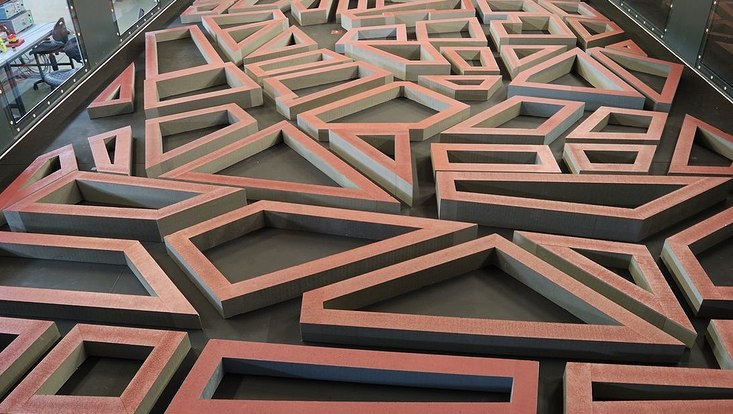
\includegraphics[width=\textwidth]{imgs/michelstad.jpg}
%         \caption{Michelstadt wind tunnel experiment (COST-M)}
%     \end{minipage}
%     \hfill
%     \begin{minipage}{0.38\textwidth}
%         \centering
%         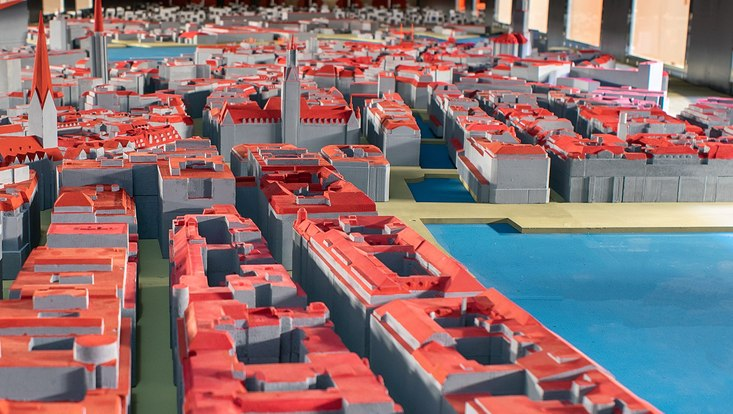
\includegraphics[width=\textwidth]{imgs/cute.jpg}
%         \caption{CUTE wind tunnel experiment (COST-C-WT) and its associated field experiment (COST-C-F).}
%     \end{minipage}
% \end{figure}

% \vspace*{-1cm}
\subsection{TURBAN Dataset}
\url{https://www.project-turban.eu/results_01_main.html}
% \vspace*{-0.2cm}\begin{figure}[h!]
%     \centering
%     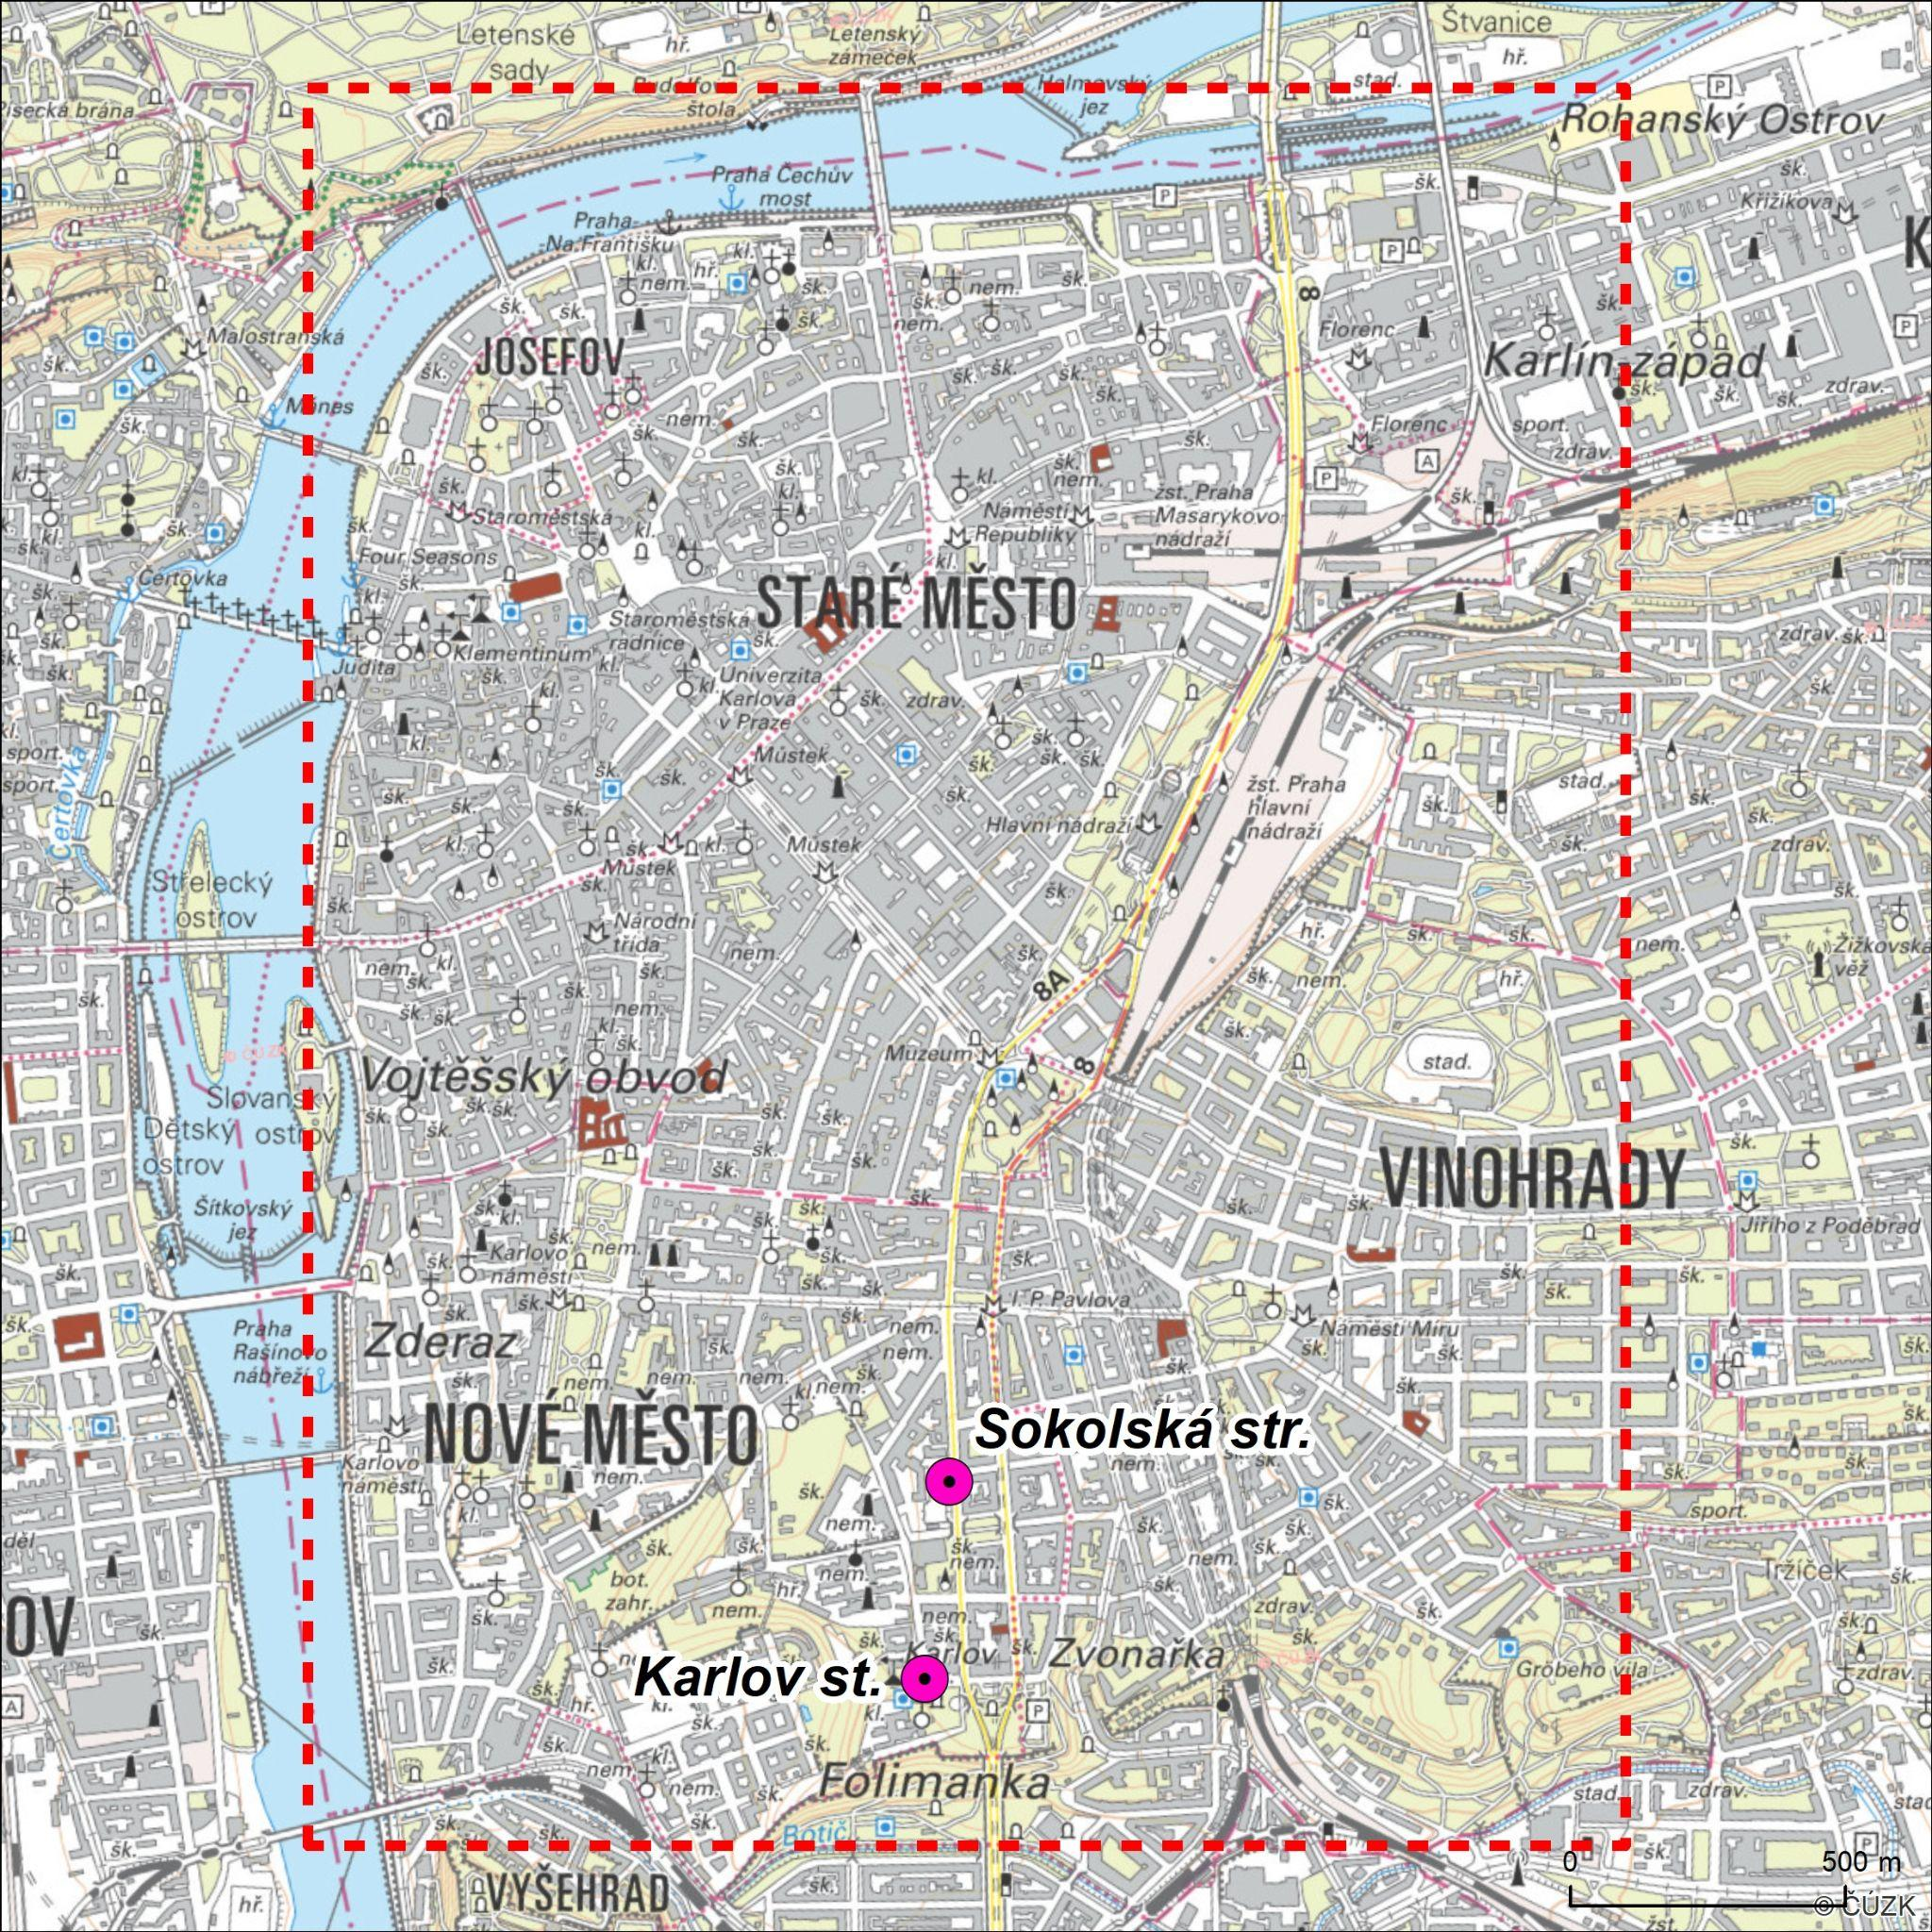
\includegraphics[scale=0.075]{imgs/turban_dataset_image.jpg}
%     \caption{Measurement campaign in the city of Prague (TURB-P)}
% \end{figure}

% \newpage


% \begin{enumerate}
%     \item \textbf{NSBL - Simple Obstacles:}
%     \begin{itemize}
%       \item[-] from AIJ Dataset: case A with single building, and case C with a street canyon (AIJ-A and AIJ-C).
%         \begin{figure}[h!]
%             \centering
%             \begin{minipage}{\dimexpr\textwidth-4cm}
%                 \begin{minipage}{0.45\textwidth}
%                     \centering
%                     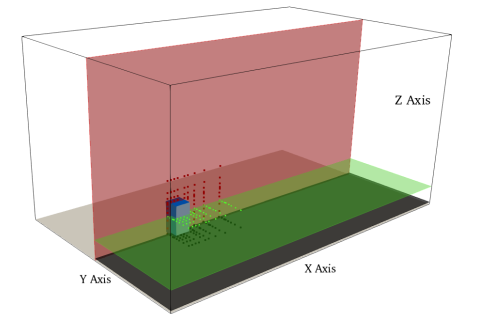
\includegraphics[width=\textwidth]{imgs/aij_A.png}
%                     \captionof{figure}{Single building in NSBL}
%                 \end{minipage}
%                 \hfill
%                 \begin{minipage}{0.45\textwidth}
%                     \centering
%                     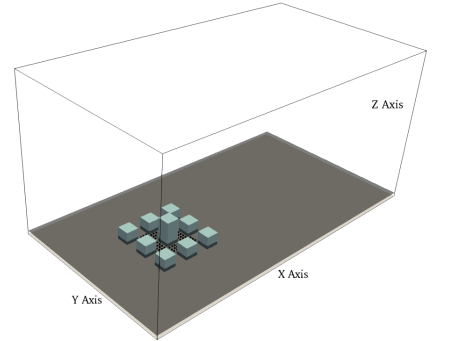
\includegraphics[width=\textwidth]{imgs/aij_C.png}
%                     \captionof{figure}{Street canyon in NSBL}
%                 \end{minipage}
%             \end{minipage}
%         \end{figure}
%         \item[-] from TPU Dataset: single building with dispersion of neutral substance (called \textit{isothermal case}, TPU-A).
%         \begin{figure}[h!]
%             \centering
%             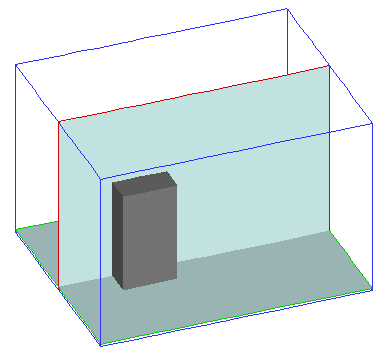
\includegraphics[width=0.35\textwidth]{imgs/tpu_1.png}
%         \end{figure}
%         \item[-] from StratEnFlo Dataset: street canyon with and without dispersion of heavy gas (NSBL configuration, SEF-B).
%             \begin{figure}[h!]
%               \centering
%               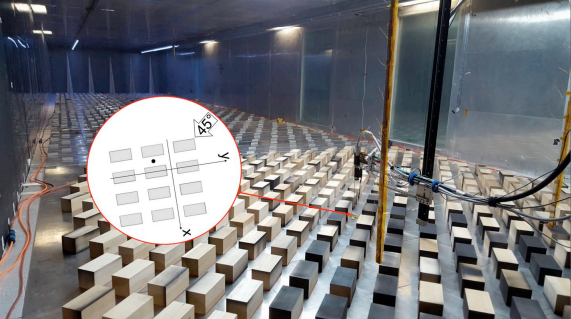
\includegraphics[scale=0.3]{imgs/sef_dataset_image.png}
%             \end{figure}
%     \end{itemize}
%     \item \textbf{NSBL - Complex Topography test cases:}
%     \begin{itemize}
%         \item from COST dataset: Cases \textit{Michelstadt} with an idealised urban geometry, and the \textit{CUTE} wind tunnel experiment with realistic representation of a European city.
%         \begin{figure}[h!]
%             \centering
%             \begin{minipage}{0.38\textwidth}
%                 \centering
%                 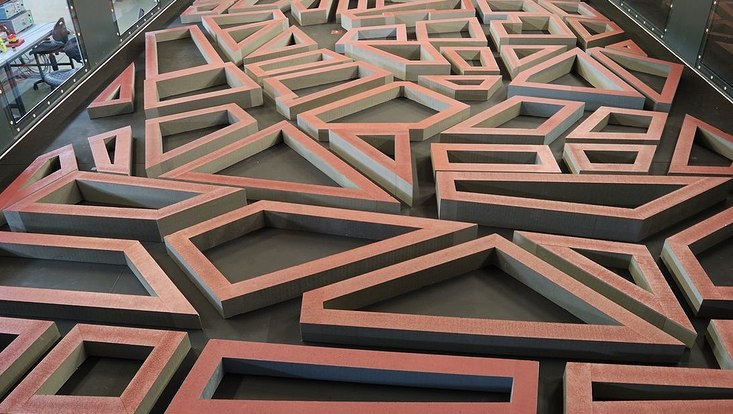
\includegraphics[width=\textwidth]{imgs/michelstad.jpg}
%                 \caption{Michelstadt wind tunnel experiment (COST-M)}
%             \end{minipage}
%             \hfill
%             \begin{minipage}{0.38\textwidth}
%                 \centering
%                 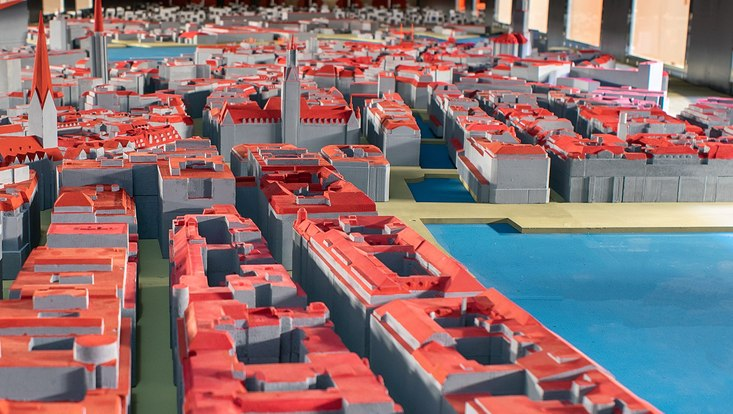
\includegraphics[width=\textwidth]{imgs/cute.jpg}
%                 \caption{CUTE wind tunnel experiment (COST-C-WT)}
%             \end{minipage}
%         \end{figure}
%     \end{itemize}
%
%     \item \textbf{SBL - Simple Obstacles test cases:}
%     \begin{itemize}
%         \item from StratEnFlo Dataset: street canyon with and without dispersion of heavy gas (SBL configuration, SEF-B).
%     \end{itemize}
%     \item \textbf{CBL - Simple Obstacles test cases:}
%     \begin{itemize}
%         \item from StratEnFlo Dataset: street canyon with and without dispersion of heavy gas (CBL configuration, SEF-C)
%         \item from TPU Dataset: single building with dispersion of neutral substance (called \textit{non-isothermal case}, TPU-B).
%         \begin{figure}[h!]
%             \centering
%             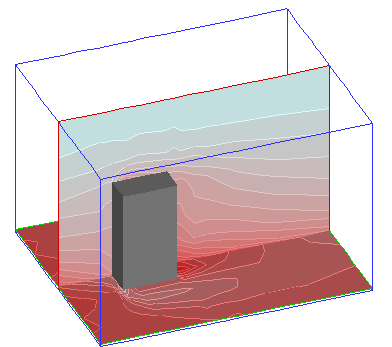
\includegraphics[width=0.4\textwidth]{imgs/tpu_2.png}
%         \end{figure}
%     \end{itemize}
%     \item \textbf{Real-world scenario test cases}
%     \begin{itemize}
%       \item COST dataset: \textit{CUTE} field experiment in a real European city (COST-C-F)
%         \begin{figure}[h!]
%             \centering
%             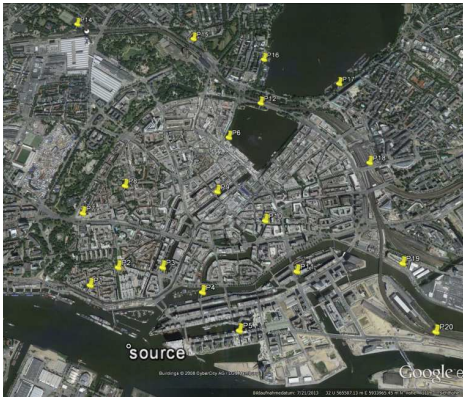
\includegraphics[width=0.4\textwidth]{imgs/cute_field_exp.png}
%             \caption{CUTE field experiment}
%         \end{figure}
%       \item TURBAN dataset: Prague field experiment (TURB-P)
%             \begin{figure}[h!]
%                 \centering
%                 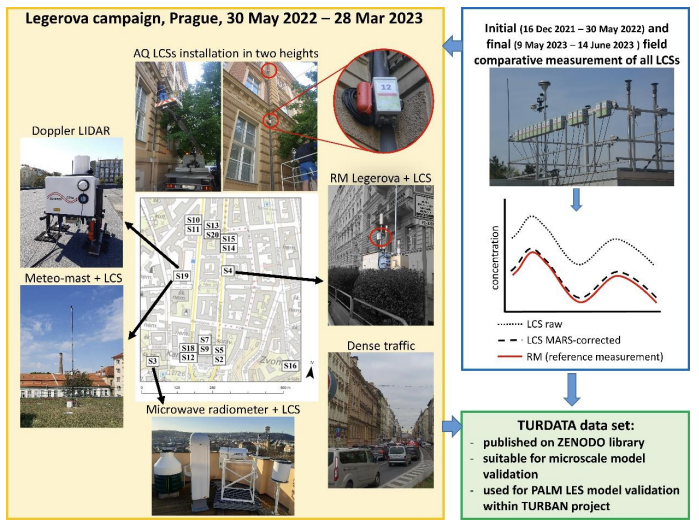
\includegraphics[width=0.4\textwidth]{imgs/turban_dataset_image.png}
%             \end{figure}
%    \end{itemize}
% \end{enumerate}
%
%




\section{Case Studies}
This section will include the description of each analyses performed, with it objectives and conclusions.\newline

Each benchmark problem is associated with experimental observations that are going to be numerically reproduced. Multi-purposes comparative analyses are defined for each test case to find the models accuracy linked to different computational strategies.\newline

Benchmarks for NSBL, SBL, and CBL configurations, refer to test cases that consider from simple-shaped obstacles to complex topography as geometry. All selected test cases address the unitary problems that characterise urban environments.\newline



In order to be able to access accuracy of computational models while providing useful results of reduced-order modelling, the validation procedure will follow 
this order: 
\begin{itemize}
    \item test cases associated with simple-shaped obstacles to not be limited by the domain sizes;
    \item test cases associated with complex topography (staying
in the wind tunnel with simplified city-like geometries)
    \item final analyses will against field experiments in a real-world urban environment (for the final step of validation/evaluation for the complete problem of microclimate simulations in urban environments) 
\end{itemize}

\subsection{Neutrally Stratified Boundary Layer (NSBL)}
                    
\subsubsection{AIJ - Case A - Single building immersed in NSBL}
    \begin{figure}[h!]
        \centering
        \hypertarget{link:aij_A}{}
        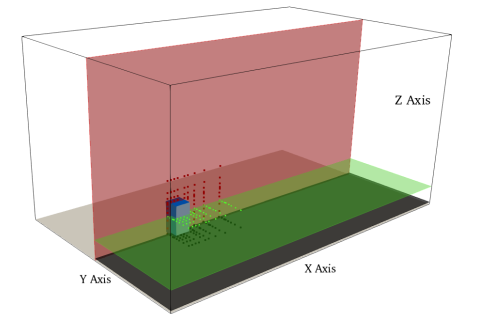
\includegraphics[scale=0.6]{imgs/aij_A.png}
        \caption{Single building immersed in NSBL}
    \end{figure}
    \textbf{Objectives:} 
    \begin{itemize}
        \item grid sensitivity analysis with steady state simulation (standard grid related analysis);
        \item from steady-state simulations to Scale Resolving Simulations (SRS), with kOmegaSSTSAS turbulence model, to highlight differences in terms of accuracy and computational cost (case-specific analysis);
        \item kOmegaSSTSAS turbulence model sensitivity analysis on the grid filter definition (case-specific analysis);
        \item SAS vs LES (case-specific analysis);
        \item development of Adaptive Mesh Refinement (AMR) criteria related to dispersion phenomena (methodology development);
        \item implementation of incremental POD for AMR (feature implementation);
        \item sensitivity analyses on turbulence models, numerical schemes, boundary conditions, and the effects of dimensionality reduction via intrusive ROM (validation-oriented study).
    \end{itemize}
    \textbf{Conclusions:} .... .\newline

\clearpage
\subsubsection{AIJ - Case C - Building blocks immersed in NSBL}
    \begin{figure}[h!]
        \centering
        \hypertarget{link:aij_C}{}
        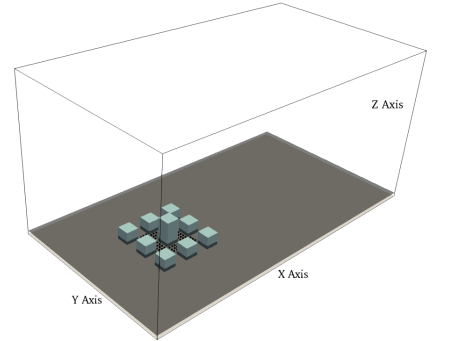
\includegraphics[scale=0.7]{imgs/aij_C.png}
        \caption{Building blocks immersed in NSBL}
    \end{figure}
    \textbf{Objectives:} ....
    \begin{itemize}
        \item grid sensitivity analysis with steady state simulation (standard grid related analysis);
        \item Application of computational methodology defined at the previous step
        \item reduced order modelling with respect changing inflow boundary conditions
        \item sensitivity analyses on turbulence models, numerical schemes, boundary conditions, and the effects of dimensionality reduction via intrusive ROM (validation-oriented study).
    \end{itemize}
    \textbf{Conclusions:} .... .\newline

\clearpage
\subsubsection{SEF - Case A - Street canyon immersed in NSBL}
    \begin{figure}[h!]
        \hypertarget{link:sef_A}{}
        \centering
        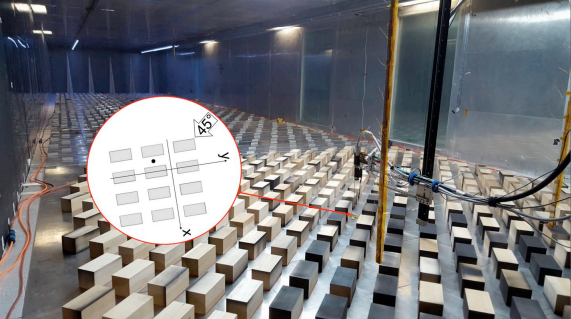
\includegraphics[scale=0.8]{imgs/sef_dataset_image.png}
        \caption{Street canyon immersed in NSBL with and without dispersion
        of heavy gas}
    \end{figure}
    \textbf{Objectives:} ....\newline
    \begin{itemize}
        \item ...
        \item ...
    \end{itemize}
    \textbf{Conclusions:} .... .\newline


\clearpage
\subsubsection{TPU - Case A - Street canyon immersed in NSBL}
    \begin{figure}[h!]
        \hypertarget{link:tpu_A}{}
        \centering
        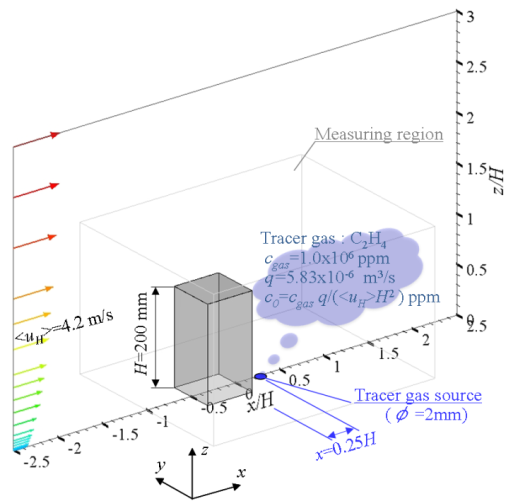
\includegraphics[scale=0.6]{imgs/tpu_dataset_image.png}
        \caption{Street canyon immersed in NSBL with and without dispersion
        of neutral gas}
    \end{figure}
    \textbf{Objectives:} ....\newline
    \begin{itemize}
        \item ...
        \item ...
    \end{itemize}
    \textbf{Conclusions:} .... .\newline

\clearpage
\subsubsection{COST-C-M - Michelstadt dataset - street canyon immersed in NSBL}
    \begin{figure}[h!]
        \hypertarget{link:cost_m}{}
        \centering
        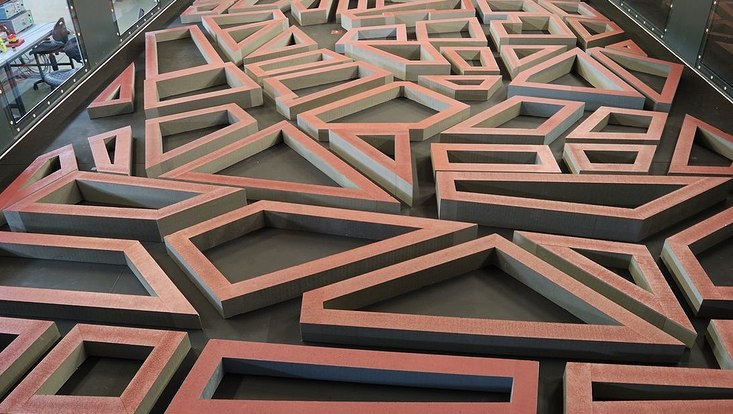
\includegraphics[scale=0.6]{imgs/michelstad.jpg}
        \caption{Street canyon immersed in NSBL}
    \end{figure}
    \textbf{Objectives:} ....\newline
    \begin{itemize}
        \item ...
        \item ...
    \end{itemize}
    \textbf{Conclusions:} .... .\newline

\clearpage
\subsubsection{COST-C-WT - COST ES 1006 CUTE dataset - wind tunnel experiment of a whole city model in NSBL}
    \begin{figure}[h!]
        \hypertarget{link:cost_c_wt}{}
        \centering
        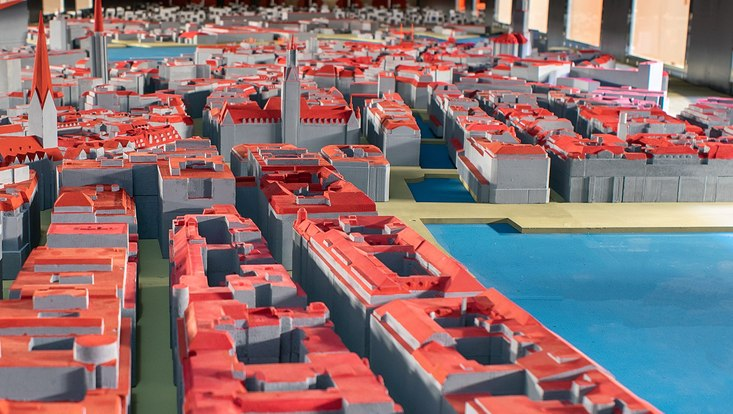
\includegraphics[scale=0.6]{imgs/cute.jpg}
        \caption{Street canyon immersed in NSBL}
    \end{figure}
    \textbf{Objectives:} ....\newline
    \begin{itemize}
        \item ...
        \item ...
    \end{itemize}
    \textbf{Conclusions:} .... .\newline


\clearpage

\subsection{Stable Boundary Layer (SBL)}

\subsubsection{SEF - Case B - Street canyon immersed in SBL}
    \begin{figure}[h!]
        \hypertarget{link:sef_A}{}
        \centering
        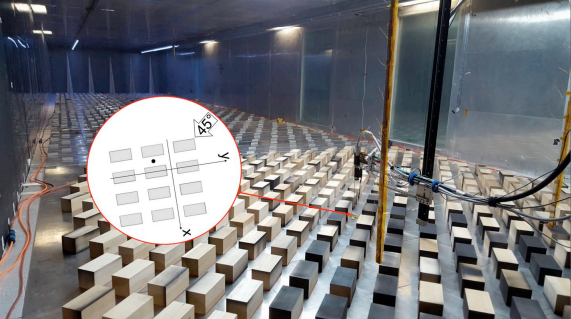
\includegraphics[scale=0.7]{imgs/sef_dataset_image.png}
        \caption{Street canyon immersed in CBL with and without dispersion
        of heavy gas}
    \end{figure}
    \textbf{Objectives:} ....\newline
    \begin{itemize}
    \item ...
    \item ...
    \end{itemize}
    \textbf{Conclusions:} .... .\newline


\clearpage
\subsubsection{TPU - Case B - Street canyon immersed in SBL}
    \begin{figure}[h!]
        \hypertarget{link:tpu_C}{}
        \centering
        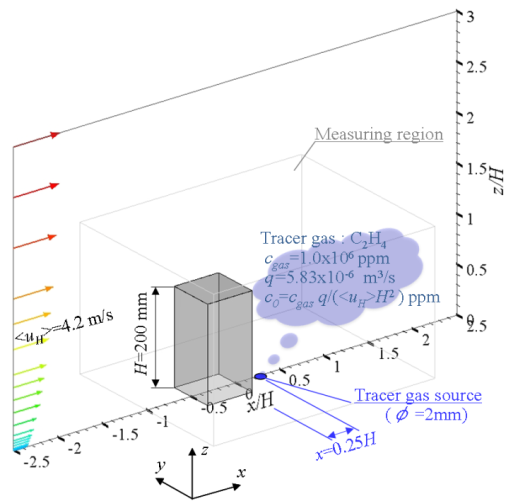
\includegraphics[scale=0.6]{imgs/tpu_dataset_image.png}
        \caption{Street canyon immersed in SBL with dispersion of neutral 
        gas}
    \end{figure}
    \textbf{Objectives:} ....\newline
    \begin{itemize}
        \item ...
        \item ...
    \end{itemize}
    \textbf{Conclusions:} .... .\newline

\clearpage

\subsection{Convective Boundary Layer (CBL)}

\subsubsection{SEF - Case C - Street canyon immersed in CBL}
    \begin{figure}[h!]
        \hypertarget{link:sef_A}{}
        \centering
        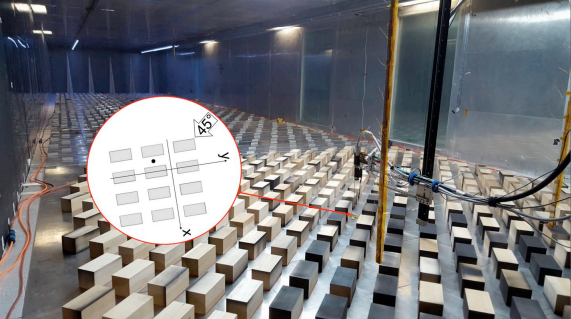
\includegraphics[scale=0.7]{imgs/sef_dataset_image.png}
        \caption{Street canyon immersed in CBL with and without dispersionof heavy gas}
    \end{figure}
    \textbf{Objectives:} ....\newline
    \begin{itemize}
    \item ...
    \item ...
    \end{itemize}
    \textbf{Conclusions:} .... .\newline


\clearpage
\subsubsection{TPU - Case C - Single building immersed in CBL}
    \begin{figure}[h!]
        \hypertarget{link:tpu_C}{}
        \centering
        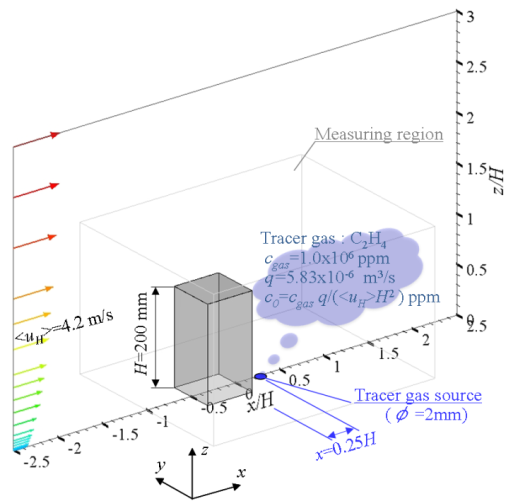
\includegraphics[scale=0.6]{imgs/tpu_dataset_image.png}
        \caption{Street canyon immersed in CBL with dispersion of neutral 
        gas}
    \end{figure}
    \textbf{Objectives:} ....\newline
    \begin{itemize}
        \item ...
        \item ...
    \end{itemize}
    \textbf{Conclusions:} .... .\newline


\clearpage

\subsection{Real-world scenario}

\subsubsection{COST-C-F - COST ES 1006 CUTE dataset - field experiment}
    \begin{figure}[h!]
        \hypertarget{link:cost_c_f}{}
        \centering
        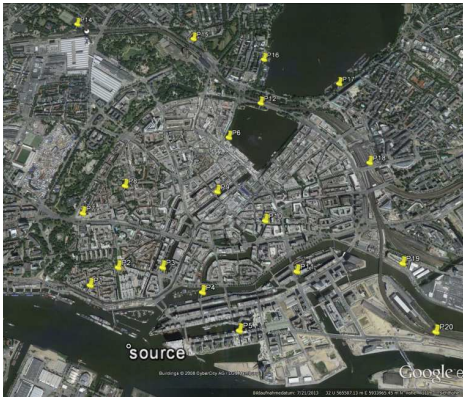
\includegraphics[scale=0.8]{imgs/cute_field_exp.png}
        \caption{Street canyon immersed in CBL with dispersion of neutral 
        gas}
    \end{figure}
    \textbf{Objectives:} ....\newline
    \begin{itemize}
        \item ...
        \item ...
    \end{itemize}
    \textbf{Conclusions:} .... .\newline


\clearpage
\subsubsection{TURB - Prague dataset - Field experiment of Prague}
    \begin{figure}[h!]
        \hypertarget{link:turb_p}{}
        \centering
        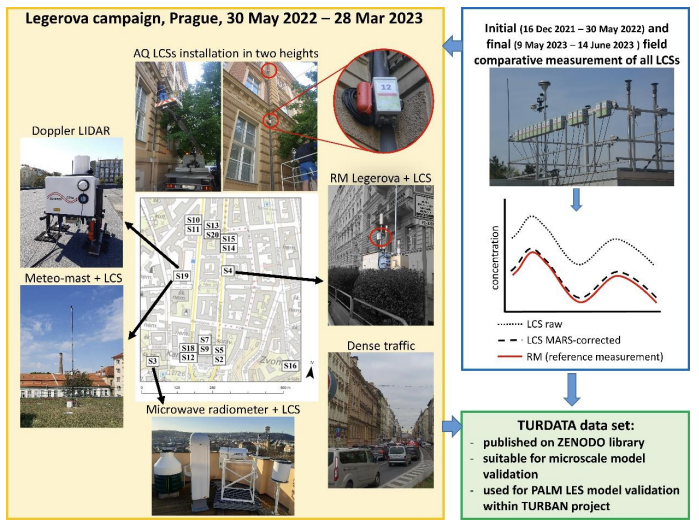
\includegraphics[scale=0.7]{imgs/turban_dataset_image.png}
        \caption{Street canyon immersed in CBL with dispersion of neutral 
        gas}
    \end{figure}
    \textbf{Objectives:} ....\newline
    \begin{itemize}
        \item ...
        \item ...
    \end{itemize}
    \textbf{Conclusions:} .... .\newline


\clearpage




\printbibliography[title={References}]

\end{document}

